\begin{nquote}{}
	*After someone sneezed* ``I used to teach engineers; when someone sneezed, the whole class would say `bless you'." - Dr. Loewen, 11/1/2023
	
	\medskip
	
	``As is the norm in mathematics, I know the name [Hausdorff] and nothing else." - Dr. Loewen, 11/1/2023
\end{nquote}

\begin{ndef}{: Metric Space}
	A \emph{\textbf{metric space}}  is a pair \((\mc{X},d)\) combining a non-empty set \(\mc{X}\) and a function \(d:\mc{X}\times \mc{X}\to \R\) obeying the conditions mentioned in the definition of a metric.
\end{ndef}
Using \(d\) for ``distance" extends ideas/notations beyond Euclidean case. For example:
\begin{equation*}
	\B[x;r)=\{x'\in\mc{X}\st d(x',x)<r\}
\end{equation*}
defines a ``ball" with centre \(x\) and radius \(r>0\). We declare a set \(\mc{U}\subseteq\mc{X}\) to be \emph{open} exactly when for all \(x\in \mc{U}\), there exists \(\eps>0\) such that \(\B[x;\eps)\subseteq \mc{U}\).
\begin{figure}[htbp]
	\centering
	\begin{tikzpicture}
		\draw[thick, dotted, black, thick, fill = white!60!gray] (0, 0.6) to [curve through ={(1.8, 0.475)..(4.75, 0.4)..(4.8, 0.02)..(5, 0)..(4.9, -0.25)..(4.75, -0.76)..(2.5, -0.72)..(0, -1)..(-1.85, -0.78)..(-1.9, -0.4)..(-2, 0)..(-1, 0.5)}] (0, 0.6);
		\node[above] at (-1.5, -0.3) {\(\mc{U}\)};
		\draw[thick, dotted, black, fill = gray!60!lightgray] (3.7, 0.3) circle (20pt);
		\node[below] at (3.7, -0.35) {\(\B[x;\eps)\)};
		\draw[fill] (3.7, 0.3) circle (1pt);
		\node[below] at (3.7, 0.3) {\(x\)};
		\draw[<->] (3.7, 0.32) -- (3.7, 1);
		\node[right] at (3.7, 0.64) {\(\eps\)};
	\end{tikzpicture}
	\caption{Visualization of an open set.}
\end{figure}
Let \(\ms{T}\) denote the set of all open sets in \(\mc{X}\) that the (metric) topology. As before, \(\B[x;\eps)\) is an open set for any \(x\in\mc{X},~\eps>0\), and the set \(\ms{T}\) has properties \((\text{HTS}~1)-(\text{HTS}~4)\).
\begin{reflection}
	As before, why do we care about this? Primarily we can think about this as a way to capture convergence of sequence ideas.
\end{reflection}
\begin{ndef}{: Convergence}
	Given a sequence \(x_1,x_2,\dots\) in \(\mc{X}\) and a point \(\hat{x}\in\mc{X}\) to say 
	\begin{equation*}
		\lim_{n\to\infty}x_n=\hat{x}~\text{or}~x_n\to\hat{x}~\text{as}~n\to\infty,
	\end{equation*}
	we say that for all \(\eps>0\), there exists \(N\in\N\) such that for all \(n>N\), \(d(x_n,\hat{x})<\eps\).
\end{ndef}
\begin{nproposition}{}
	In a metric space \((\mc{X},d)\), a set \(\mc{U}\) is open iff every point \(x\in\mc{U}\) obeys the following: whenever any \(x_n\) has \(x=\displaystyle\lim_{n\to\infty}x_n\) then \(x_n\in\mc{U}\) for all \(n\) sufficiently large. 
\end{nproposition}
\begin{proof}
	\((\Rightarrow)\) Given \(\mc{U}\in\ms{T}\) and a point \(x\in\mc{U}\), definition of open set gives some \(\eps>0\) such that \(\B[x;\eps)\subseteq\mc{U}\). So, if \((x_n)\) is any sequence with \(x_n\to x\), definition of convergence gives \(N\in\N\) such that for all \(n>N\), \(d(x_n,x)<\eps\), where \(x_n\in\B[x;\eps)\subseteq\mc{U}\).
	
	\medskip
	
	\((\Leftarrow)\) We prove this by contrapositive; assume set \(\mc{U}\) is \emph{not} open. Then some \(x\in\mc{U}\) breaks the defining property: there exists \(\eps>0\), \(\B[x;\eps)\subseteq\mc{U}\). So, for each \(n\in\N\), \(\eps=\displaystyle\frac{1}{n}\) here makes \(\B\left[x;\displaystyle\frac{1}{n}\right)\not\subseteq\mc{U}\). That is, some point \(x_n\in\B\left[x;\displaystyle\frac{1}{n}\right)\) obeys \(x_n\notin\mc{U}\). Now \(d(x_n,x)<\displaystyle\frac{1}{n}\) (an ``analogue" of the Squeeze theorem in \(\R\)), so sequence \(x_n\) obeys \(x_n\to x\) and \(x_n\notin\mc{U}\).
\end{proof}
\begin{note}
	This is one of the pros of doing the course not in the same order as Rudin; we get many concrete examples for dealing with convergence, so metric spaces make a lot more sense.
\end{note}

\subsection{Ball shapes in \(\R^2\)}
Note that \(\R^2=\{x=(x_1,x_2):{x_1,x_2\in\R}\}\) can be given several metrics, some of which are:
\begin{itemize}
	\item \(d_2(x,y)=\sqrt{(x_1-y_1)^2+(x_2-y_2)^2}\); we recover the most popular ball \(\B[0;1)\):
	\begin{figure}[htbp]
		\centering
		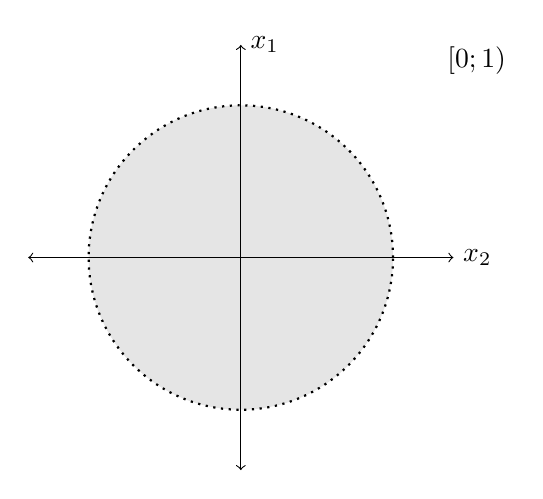
\begin{tikzpicture}
			\draw[dotted, thick, fill = white!60!lightgray] (0, 0) circle (55pt);
			\draw[<->] (0,-2.7) -- (0,2.7);
			\draw[<->] (-2.7,0) -- (2.7,0);
			\node[right] at (2.7,0) {\(x_2\)};
			\node[right] at (0,2.7) {\(x_1\)};
			\node[right] at (2.5,2.5) {\(\B[0;1)\)};
		\end{tikzpicture}
		\caption{The \(\B[0;1)\) ball; it is actually a ball in this case.}
	\end{figure}
	
	\item \(d_1(x,y)=|x_1-y_1|+|x_2-y_2|\); our ball is now shaped like a diamond:
	\begin{figure}[htbp]
		\centering
		\begin{tikzpicture}
			\node[diamond,draw, dotted, thick, fill=white!60!lightgray, minimum width= 3cm, minimum size= 3cm, minimum height= 3cm] (d) at (0,0) {};
			\draw[<->] (0,-2) -- (0,2);
			\draw[<->] (-2,0) -- (2,0);
			\node[right] at (2,0) {\(x_2\)};
			\node[right] at (0,2) {\(x_1\)};
			\node[right] at (1,1) {\(\B[0;1)\)};
		\end{tikzpicture}
		\caption{The \(\B[0;1)\) ball; it is a diamond in this case.}
	\end{figure}
	\begin{comment}
		\draw[<->] (0,-2.7) -- (0,2.7);
		\draw[<->] (-2.7,0) -- (2.7,0);
		\draw[-, dotted, thick] (0, 2) -- (2, 0);
		\draw[-, dotted, thick] (2, 0) -- (0, -2);
		\draw[-, dotted, thick] (0, -2) -- (-2, 0);
		\draw[-, dotted, thick] (-2, 0) -- (0, 2);
	\end{comment}
	
	\item \(d_{\infty}(x,y)=\text{max}\{|x_1-y_1|,|x_2-y_2|\}\); our ball is now a square:
	\begin{figure}[H]
		\centering
		\begin{tikzpicture}[square/.style={regular polygon,regular polygon sides=4}]
			\node[square, draw, dotted, thick, fill=white!60!lightgray, minimum width= 3cm, minimum size= 3cm, minimum height= 3cm] (s) at (0,0) {};
			\draw[<->] (0,-2) -- (0,2);
			\draw[<->] (-2,0) -- (2,0);
			\node[right] at (2,0) {\(x_2\)};
			\node[right] at (0,2) {\(x_1\)};
			\node[right] at (1.3,1.3) {\(\B[0;1)\)};
		\end{tikzpicture}
		\caption{The \(\B[0;1)\) ball; it is a square in this case.}
	\end{figure}
	
	\item Can interpolate: \(d_p(x,y)=(|x_1-y_1|^p+|x_2-y_2|^p)^{1/p}\), which is a valid metric for any \(p\geq 1\), including \(p=+\infty\).
\end{itemize}
In principle, each different metric gives a different family of open sets, and different story with convergence. However, it is quite bizarre that they all define a compatible idea of convergence: the set of open set are the same regardless of the metric.

\subsection{Hausdorff topological space}
\begin{ndef}{}
	A HTS is an ordered pair \((\mc{X},\ms{T})\) where \(\mc{X}\) is a nonempty set, and \(\ms{T}\subseteq\ms{P}(\mc{X})\) with these 4 properties:
	\begin{enumerate}[(HTS 1)]
		\item \(\emptyset\in\ms{T},~\mc{X}\in\ms{T}\).
		
		\item For any collection \(\mc{J}\subseteq\ms{T}\) one has \(\displaystyle\bigcup\mc{J}\in\ms{T}\) (any union of open sets is open.)
		
		\item If \(\mc{U}_1,\dots,\mc{U}_N\in\ms{T}\) (and \(N\in\N\)) then \(\displaystyle\bigcap_{k=1}^N\mc{U}_k\in\ms{T}\) (any finite intersection of open sets in open.)
		
		\item Whenever \(x\neq y\) in \(\mc{X}\), there exists \(\mc{U},\mc{V}\in\ms{T}\) obeying \(x\in\mc{U},~y\in\mc{V}\), and \(\mc{U}\cap \mc{V}=\emptyset\) (enough open sets to separate points.)
	\end{enumerate}
\end{ndef}

\begin{example}~
	\begin{itemize}
		\item Any metric topology.
		
		\item Discrete topology: \(\ms{T}=\ms{P}(\mc{X})\) (``every set if open".)
	\end{itemize}
\end{example}